\documentclass[10pt,a4paper]{article}
\usepackage{lmodern}
\newcommand{\codefont}{\fontsize{8}{9.5}\selectfont\ttfamily}
\usepackage[spanish,es-nodecimaldot]{babel}
\usepackage{amsmath,amssymb,booktabs,array,geometry,graphicx,xcolor,listings,float,etoolbox,hyperref}
\geometry{margin=1.8cm}
\setlength{\parindent}{0pt}
\setlength{\parskip}{3.5pt}
\setlength{\abovedisplayskip}{5pt}
\setlength{\belowdisplayskip}{5pt}

\definecolor{azul}{HTML}{245B91}

\pagestyle{plain}

\hypersetup{
  colorlinks=true,
  linkcolor=azul,
  urlcolor=azul,
  pdftitle={Trabajo Final}
}
\setcounter{tocdepth}{1}
\setcounter{secnumdepth}{0}

\newcommand{\BetaDist}{\operatorname{Beta}}
\newcommand{\Bin}{\operatorname{Bin}}
\newcommand{\Unif}{\operatorname{Unif}}
\newcommand{\Nor}{\operatorname{N}}
\newcommand{\Var}{\operatorname{Var}}
\newcommand{\DIC}{\operatorname{DIC}}

\newcommand{\inciso}[1]{\par\smallskip\textbf{#1}\quad}
\newcommand{\etapa}[1]{\par\smallskip\textbf{#1.}\quad}

\lstset{
  language=R,
  basicstyle=\codefont,
  keywordstyle=\codefont,
  stringstyle=\codefont,
  backgroundcolor=\color{black!3},
  frame=none,
  rulecolor=\color{black!15},
  breaklines=true,
  showstringspaces=false,
  columns=fullflexible,
  keepspaces=true,
  commentstyle=\color{black!55},
  xleftmargin=6pt,
  xrightmargin=6pt,
  aboveskip=6pt,
  belowskip=8pt,
  literate={á}{{\'a}}1 {é}{{\'e}}1 {í}{{\'i}}1 {ó}{{\'o}}1 {ú}{{\'u}}1
           {Á}{{\'A}}1 {É}{{\'E}}1 {Í}{{\'I}}1 {Ó}{{\'O}}1 {Ú}{{\'U}}1
           {ñ}{{\~n}}1 {Ñ}{{\~N}}1 {ü}{{\"u}}1 {Ü}{{\"U}}1
}

% Líneas de analisis.R resaltadas en el Anexo A: posterior, muestra, DIC y phi elegido.
% Son números de línea del archivo: si cambia el código, hay que actualizarlos.
\definecolor{resaltado}{HTML}{FFEE99}
\newcommand{\lineasresaltadas}{}
\forcsvlist{\listadd\lineasresaltadas}{22,24,26,27,28,38}
\newcommand{\resaltarlinea}[1]{%
  \xifinlist{#1}{\lineasresaltadas}%
    {\rlap{\smash{\color{resaltado}\rule[-2.85pt]{\linewidth}{9.5pt}}}}{}%
}

\begin{document}

{\Large\bfseries Trabajo Final}\hfill Inferencia II, 2026
\par\smallskip
\textbf{Artículo analizado:} Bon, J. J. \emph{et al.} (2023), ``Being Bayesian in the 2020s: opportunities and challenges in the practice of modern applied Bayesian statistics'', \emph{Philosophical Transactions of the Royal Society A}, 381: 20220156 (\url{https://doi.org/10.1098/rsta.2022.0156}).\\
\textbf{Integrantes:} Florencia Cosentino, Miguelángel Díaz
\par\medskip

\section{1. Ideas principales del artículo}\label{sec:ideas}

El artículo es un resumen de cómo se puede adaptar la inferencia bayesiana cuando el muestreo MCMC deja de ser suficiente. Esto debido a que en muchos de los problemas nuevos que están surgiendo MCMC no es suficiente, porque los datos pueden ser costosos, y podemos tener múltiples fuentes con distinto comportamiento y bajo problemas más administrativos o políticos. Esto conlleva a que la verosimilitud esté dada por simulaciones sin densidades explícitas o podamos tener pocas observaciones. Para abordar esto se muestran seis ejemplos de problemas de aplicaciones reales y se resuelven manteniendo el modelado bayesiano.

\begin{itemize}
\item En la Sección 2 se muestra un ejemplo en el que hay un problema de recolección de datos para monitorear barreras de coral, proponiendo distintas técnicas para optimizar el experimento muestreando de forma inteligente.
\item En la Sección 3 se tienen fuentes de datos de distinto origen y se proponen modelos que intentan separar lo que se desea medir de la realidad de lo que introduce el ser humano al medirla.
\item En la Sección 4 explican cómo analizar datos que están repartidos entre distintas instituciones con el atlas australiano de cáncer. Dado que los hospitales no quieren proveer los datos porque son confidenciales y se entrena un modelo.
\item En la Sección 5 se tienen datos del volumen de tumores a lo largo del tiempo. El objetivo es estudiar su crecimiento. El problema es que no pueden calcular la verosimilitud de forma sencilla porque el crecimiento del tumor depende de muchas acciones individuales y aleatorias de las células. Entonces, para un valor de $\theta$, simulan el crecimiento del tumor y comparan los resultados con los datos observados. Repiten esto para distintos valores de $\theta$ para identificar cuáles son compatibles con los datos.
\item En la Sección 7 se muestra la importancia de implementar estos modelos en aplicaciones y software reproducible para facilitar la interpretación y el uso práctico de los resultados.
\end{itemize}

Nosotros elegimos trabajar más a detalle la Sección 6, en la que se aborda la transferencia de modelos entre un dominio fuente $S$ y un dominio final $T$. Esto con el objetivo de solucionar el problema de tener pocos datos en $T$. El marco de trabajo es encuestas ecológicas en distintas zonas de la Antártida, regulando cuánto peso recibe la fuente para no degradar las estimaciones si ambos dominios difieren mucho.

\section{2. Resultado central}\label{sec:resultado}

\begin{quote}
``This flattening is done by choosing a value $\phi\in[0,1]$ and raising the source likelihood to the value of $\phi$ which gives
\[
\pi(\theta\mid\phi,y_T,y_S)\propto f_T(y_T\mid\theta)f_S(y_S\mid\theta)^{\phi}\pi(\theta),
\]
where $f_S(y_S\mid\theta)$ and $f_T(y_T\mid\theta)$ are the source and target likelihood functions, respectively.''
\end{quote}

{\small Bon \emph{et al.} (2023), sección 6, p.~16.}

Cuando $\phi = 0$, $[f_S(y_S\mid\theta)]^0 = 1$, y la posterior depende solo de los datos de $T$ y de la previa. La inferencia descarta por completo los datos de la fuente. Si $\phi = 1$, se utiliza verosimilitud fuente con el mismo peso que la del objetivo, como si fuese posible ampliar los datos de $T$ incorporando las de $S$. Luego, para valores intermedios $0 < \phi < 1$, si se considera la log-verosimilitud fuente, esta queda multiplicada por $\phi$ y se pondera la influencia de $S$.

Si ambos dominios son similares, entonces un $\phi$ alto puede mejorar la precisión de las estimaciones en $T$, ya que se incorpora información relevante al modelo por otro lado, si difieren, puede sesgarlas y producir ``negative transfer'' o transferencia negativa.

\pagebreak
Para elegir $\phi$, se presentan dos alternativas:
\begin{itemize}
\item Asignarle una previa $\phi\sim\Unif(0,1)$ y obtener su posterior junto con la de $\theta$. Esto requiere normalizar la \emph{power prior} para cada $\phi$, lo que puede ser costoso. Además, los autores señalan que la posterior de $\phi$ suele diferir poco de su previa, por lo que los datos aportan poca información para elegirlo.
\item La otra opción es hacer un grid search con valores de $\phi$ y elegir con algún criterio, en el paper se menciona el criterio de información de devianza ($\DIC$), calculado solo con los datos de $T$.
\end{itemize}

\section{3. Conexión con los contenidos del curso}\label{sec:conexion}

\etapa{Previas Conjugadas}\\
\textbf{1.} Podemos aplicar la fórmula del artículo al modelo Beta-Binomial visto en el curso.

$$\theta\sim\BetaDist(a_0,b_0)$$
\[
\pi(\theta)=\frac{\theta^{a_0-1}(1-\theta)^{b_0-1}}{B(a_0,b_0)},
\qquad
f_j(y_j\mid\theta)=\binom{n_j}{y_j}\theta^{y_j}(1-\theta)^{n_j-y_j},
\quad j\in\{S,T\},
\]
donde $B$ es la función beta y $0<\theta<1$.

\textbf{2.} Para cada valor de $\phi$ que probamos, se tiene según el paper:
\[
\begin{aligned}
\pi(\theta\mid y_T,y_S,\phi)
&\propto f_T(y_T\mid\theta)\,[f_S(y_S\mid\theta)]^\phi\,\pi(\theta)\\
&=\binom{n_T}{y_T}\theta^{y_T}(1-\theta)^{n_T-y_T}
\left[\binom{n_S}{y_S}\theta^{y_S}(1-\theta)^{n_S-y_S}\right]^\phi
\frac{\theta^{a_0-1}(1-\theta)^{b_0-1}}{B(a_0,b_0)}.
\end{aligned}
\]

\textbf{3.} Al elevar la verosimilitud fuente a $\phi$, sus exponentes quedan multiplicados por $\phi$.

Entonces:
\[
\begin{aligned}
\pi(\theta\mid y_T,y_S,\phi)
&\propto \theta^{y_T}(1-\theta)^{n_T-y_T}
\theta^{\phi y_S}(1-\theta)^{\phi(n_S-y_S)}
\theta^{a_0-1}(1-\theta)^{b_0-1}\\
&=\theta^{a_0+y_T+\phi y_S-1}
(1-\theta)^{b_0+n_T-y_T+\phi(n_S-y_S)-1}.
\end{aligned}
\]

\textbf{4.} Comparando los exponentes con los de la densidad Beta, la posterior es:
\[
\theta\mid y_T,y_S,\phi \sim \BetaDist\bigl(a_0 + \phi y_S + y_T,\; b_0 + \phi(n_S-y_S) + n_T-y_T\bigr).
\]
Donde ya se sabe, por los resultados vistos en el teórico, que si consideramos solo los datos de T, nos queda:
\[
\theta\mid y_T \sim \BetaDist\bigl(a_0 + y_T,\; b_0 + n_T-y_T\bigr).
\]

Por lo tanto, sumamos los éxitos al primer parámetro y los fracasos al segundo de la misma forma que en la vista en el curso. La diferencia es que los de $S$ se ponderan por $\phi$.

\etapa{Aproximación por grilla y Monte Carlo}
En el Práctico 2 vimos aproximación por grilla y Monte Carlo. En nuestro ejemplo usamos una grilla de $\phi$ para probar cuánto peso darle a la fuente y otra de $\theta$ para aproximar la posterior. Para cada valor de $\phi$, evaluamos la fórmula del artículo desarrollada arriba en los puntos de la grilla de $\theta$ y dividimos los resultados por su suma. Así obtenemos probabilidades con las que sorteamos valores de $\theta$. Con esas muestras calculamos la media posterior y el $\DIC$. Repetimos el procedimiento para cada $\phi$ y elegimos el de menor $\DIC$.

%\etapa{Comparación con DIC}
%El $\DIC$, visto en el Tema 10, combina el ajuste a los datos con una %penalización por la complejidad del modelo. Para cada $\phi$, calculamos la %devianza usando solo los datos del objetivo:
%\[
%D(\theta) = -2\log f_T(y_T\mid\theta),
%\qquad
%\DIC = 2\,\overline{D(\theta)} - D(\bar{\theta}).
%\]
%Aquí, $\overline{D(\theta)}$ es el promedio de las devianzas calculadas con las muestras posteriores y $\bar{\theta}$ es la media de esas muestras. Elegimos el $\phi$ con menor $\DIC$. Usar siempre los datos de $T$ permite comparar las opciones sobre el mismo conjunto de datos.

\section{4. Ejemplo en R}\label{sec:ejemplo}

Fijamos $T$ con $6$ éxitos de $20$ ensayos ($30\%$) y $S$ de $100$ observaciones. Usamos una previa $\theta\sim\BetaDist(1,1)$ y variamos el número de éxitos de $S$. Una vez elegimos un $S$ nuevo, probamos valores de $\phi$ entre $0$ y $1$, con paso $0.1$ y aproximamos como vimos en el Práctico 2. Con esas muestras calculamos el $\DIC$ y elegimos el menor. Cuando la fuente está cerca del $30\%$, el criterio permite incorporarla completa. Con $S=28\%$, $29\%$, $31\%$ o $32\%$, el criterio elige $\phi=1$. Al aumentar la diferencia aparecen pesos intermedios, por ejemplo, con $S=18\%$ o $44\%$, se elige $\phi=0.3$. El Cuadro~\ref{tab:sensibilidad} muestra algunos valores.

\begin{table}[H]
\centering
\small
\begin{tabular}{@{}cc@{}}
\toprule
\textbf{Fuente (\%)} & $\phi^*$ \\
\midrule
6 & 0.0 \\
7 & 0.1 \\
18 & 0.3 \\
28 & 1.0 \\
29 & 1.0 \\
30 & 1.0 \\
31 & 1.0 \\
32 & 1.0 \\
44 & 0.3 \\
54 & 0.0 \\
60 & 0.0 \\
\bottomrule
\end{tabular}
\caption{Peso elegido por grilla y Monte Carlo para algunos valores del barrido.}
\label{tab:sensibilidad}
\end{table}

Los primeros ceros aparecen en $6\%$ y $54\%$, respectivamente.

\begin{figure}[H]
\centering
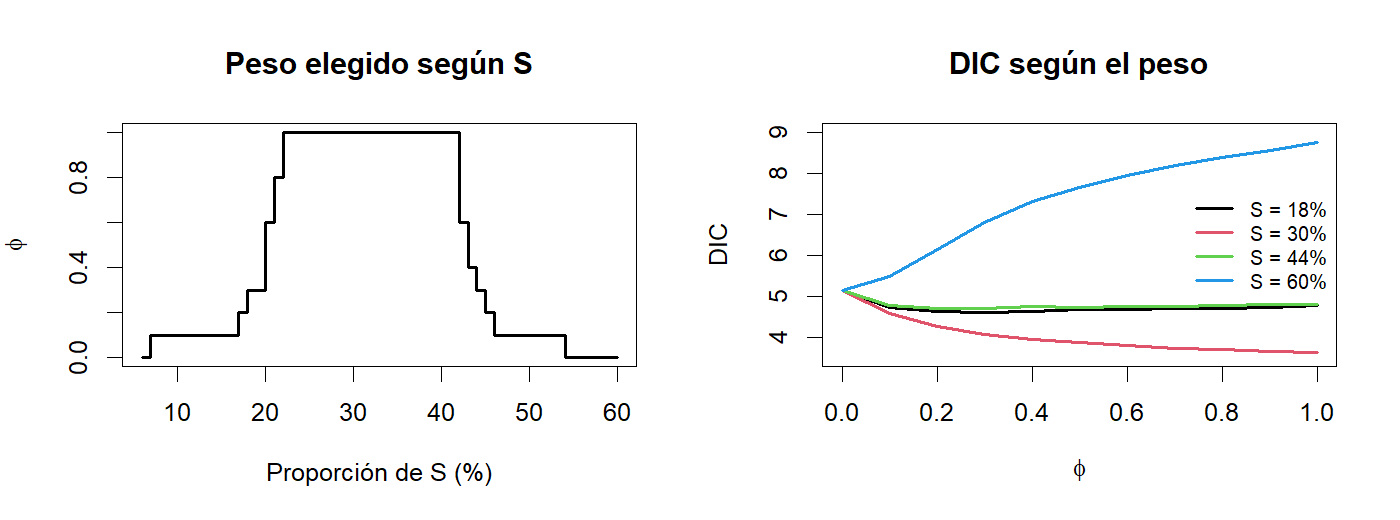
\includegraphics[width=0.95\linewidth]{figuras/sensibilidad-fuente.png}
\caption{Izquierda: peso elegido al variar $S$. Derecha: evolución del $\DIC$ para cuatro valores del mismo barrido.}
\label{fig:sensibilidad}
\end{figure}

\section{5. Valoración crítica y limitaciones del enfoque}\label{sec:critica}

El principal limitador es que tenemos que saber asignar bien $\phi$. Al asignarle una previa no estamos garantizando que los datos permitan estimarlo con precisión, sin embargo, los autores advierten que su posterior puede cambiar poco respecto de la previa. Además, los intervalos posteriores no van a incorporar la incertidumbre de $\phi$ porque luego de que aplicamos la grilla, lo damos por conocido. Finalmente, más a nivel general del artículo, vemos que no ofrece una comparación de todos los métodos.

\section{6. Partes que necesitamos estudiar más}\label{sec:nocomprendido}

\begin{itemize}
\item Como nos centramos en la transferencia de modelos, nos falta estudiar con más detalle los otros métodos para entender cómo funcionan y cuándo se pueden aplicar.
\item Deberíamos estudiar mejor cómo se calcula el $\DIC$ y cuáles son sus limitaciones para elegir $\phi$. También nos queda investigar más a fondo si la transferencia aporta mejoras en algún problema con datos reales.
\end{itemize}

\clearpage
\section{7. Trabajo con IA}\label{sec:ia}

\etapa{Parte a: resumen y evaluación}
Le pedimos a la IA un resumen breve de la sección 6 del artículo, con acceso al repositorio local y al PDF. La respuesta identifica correctamente el objetivo de transferir información desde una fuente con más datos hacia un dominio objetivo con pocos datos. También explica los extremos $\phi=0$ y $\phi=1$, el riesgo de transferencia negativa y la dificultad de aprender el peso a partir de los datos.

Hay al menos dos aspectos para agregar al resumen. Primero, el pedido se centró en la sección 6 y, por eso, la respuesta no resume el artículo completo: falta situar la transferencia junto con las otras aplicaciones y desafíos que describimos en la \hyperref[sec:ideas]{Sección 1}. Segundo, falta precisar la elección del peso mediante una grilla y el $\DIC$ calculado solo con los datos de $T$, así como distinguir ese procedimiento de asignar una previa a $\phi$. Incorporamos esta explicación en la \hyperref[sec:resultado]{Sección 2}. El prompt y la respuesta se adjuntan en el \hyperref[anexo:ia]{Anexo B}.

\etapa{Parte b: uso como tutor}
Le pedimos simplificar la transferencia entre dominios y la elección de $\phi$. La explicación ayudó a entender cómo se regula la influencia de la fuente. La IA introdujo la expresión «transferencia positiva» y repreguntamos si aparecía en el artículo. Contrastamos la respuesta con la sección 6, página 16: los autores mencionan explícitamente la «transferencia negativa» cuando la información de la fuente perjudica la inferencia o la predicción. La repregunta y la corrección se incluyen en el anexo.

\etapa{Parte c: ejemplo en R}
También usamos la IA para generar y ajustar el ejemplo Beta--Binomial en R base. Le indicamos que consultara la consigna, el artículo, los prácticos, los talleres y las diapositivas del repositorio local. En particular, el Práctico 2 sirvió de referencia para la aproximación por grilla y Monte Carlo. Las instrucciones se precisaron mediante intercambios y correcciones para mantener la coherencia entre código, resultados y explicación.

El script \path{analisis.R} calcula el $\DIC$ para cada fuente y cada peso, y genera la figura y la salida numérica. El anexo incluye el código y los extractos de la interacción. El ejemplo permite estudiar cómo cambia la selección de $\phi$; no constituye una validación del método con datos reales.

\clearpage
\section{Anexo}\label{sec:anexo}

\subsection{Anexo A: código en R y salidas numéricas}\label{anexo:codigo}

\lstinputlisting[numbers=left,numbersep=0pt,numberstyle=\resaltarlinea]{analisis.R}

\clearpage
Salida de consola del experimento de fuente variable con aproximación por grilla ($99$ puntos en $[0.01,0.99]$, $10000$ muestras, semilla \texttt{84735}):

\lstinputlisting[language={},backgroundcolor=\color{white}]{resultados/salida-power-prior.txt}

\clearpage
\subsection{Anexo B: Uso de IA}\label{anexo:ia}

\etapa{\textbf{Parte a:}}

Prompt usado (Terra 6.1 High):

\noindent\fbox{%
\begin{minipage}{\dimexpr\linewidth-2\fboxsep-2\fboxrule\relax}
\setlength{\parindent}{0pt}
\setlength{\parskip}{0.7em}

Dame un resumen breve, completo y conciso de la sección seis del artículo elegido para la tarea final.
Revisa el repositorio local para entender el contexto. Tienes disponible el artículo en formato PDF.

\end{minipage}%
}

Respuesta:

\noindent\fbox{%
\begin{minipage}{\dimexpr\linewidth-2\fboxsep-2\fboxrule\relax}
\setlength{\parindent}{0pt}
\setlength{\parskip}{0.7em}

La sección 6 de \emph{Being Bayesian in the 2020s} trata sobre la
\textbf{transferencia de modelos}: aprovechar información de un dominio
\textbf{fuente}, donde hay suficientes datos, para mejorar la inferencia
en un dominio \textbf{objetivo}, donde son escasos. El desafío es decidir
\textbf{cuándo, qué y cómo transferir}.

Usar toda la información de la fuente puede ser perjudicial si ambos
dominios son distintos: esto se conoce como \textbf{transferencia negativa}.
Una alternativa son las \emph{power priors}, que elevan la verosimilitud
de la fuente a una potencia \(\phi\) entre 0 y 1. Con \(\phi=0\) no se
transfiere información; con \(\phi=1\) se usa toda.

Los autores también mencionan métodos que seleccionan o ponderan datos
de la fuente, así como procesos gaussianos que controlan la relación entre
dominios. Identifican un problema abierto: \textbf{elegir cuánto transferir
e incorporar la incertidumbre sobre esa elección}. Por ejemplo, asignar
una distribución previa a \(\phi\) no garantiza que los datos permitan
aprender mucho sobre su valor. Proponen avanzar hacia métodos bayesianos
más generales, aplicables a distintos tipos de modelos.

Fuente: sección 6, páginas 16–17
\end{minipage}%
}

\subsection*{Repregunta sobre la terminología}


\begin{quote}
\textbf{IA:} «Si ambos dominios son similares respecto de $\theta$, incorporar datos de $S$ puede mejorar la precisión de las estimaciones en $T$: esto se llama transferencia positiva. […]»

\textbf{Usuario:} «se menciona eso de transferencia positiva?»

\textbf{IA:} «No. En la sección 6, Bon \emph{et al.} explican que usar información de la fuente puede mejorar la inferencia en el dominio objetivo, pero \textbf{no llaman a eso “transferencia positiva”}. Sí usan el término \emph{transferencia negativa} cuando las diferencias entre dominios perjudican la inferencia o la predicción. […]»
\end{quote}



\end{document}
